\documentclass[spanish]{udpreport}
\usepackage[utf8]{inputenc}
\usepackage[spanish]{babel}

% Podemos establecer el logo de alguna entidad o dejar el de la UDP (defecto)
%\setlogo{EITFI}

\title{Informe de redes de datos 4\\
"STP y VLAN "\\}
\author{Alumno: Camilo Araya \\ Javiera Araya
\\Profesor: Nicolás Hidalgo\\Ayudante: Martín Griño}
\date{\today}



\begin{document}
\maketitle

\chapter*{Resumen} 
\addcontentsline{toc}{section}{Resumen} 
\markboth{RESUMEN}{RESUMEN} 
El presente informe tiene por objetivo implementar los dos protocolos, estos protocolos están orientados al uso de Switch como eje central, dichos protocolos serán STP y VLAN, para abordar de manera efectiva su funcionamiento y diferencia, se hará uso de la herramienta de simulación de redes Cisco Packet Tracer, de manera tal que para esta experiencia deberán configurarse los equipos con las indicaciones para cada protocolo y ver su funcionamiento.

\tableofcontents
\chapter{Introducción}
Hay ocasiones en que en una red implementada existan problemas de congestión debido a la redundancia de esta, los cuales en algunos casos puede generar problemas (ocacionado principalmente por los loops), para ello se tiene que en los Switches existen protocolos con el fin de descongestionar o bien lograr una mejor administración de la red, estos protocolos se mencionaran a continuación:
\section{STP}
Spanning Tree Protocol que en siglas se denomina STP un protocolo de capa 2 que se ejecuta en Bridges y Switches, la especificación es IEEE 802.1D. El objetivo de STP es garantizar que no se creen loops al armar una red que tenga trayectorias redundantes.
\section{VLAN}
Virtual LAN que en siglas es VLAN es un metodo para crear redes logicas independientes dentro de una misma red fisica, el objetivo de esto es aliviar la sobrecarga ejercida en el switch al momento de tener una red con trayectorias redundantes.

\chapter{Desarrollo}
Como se menciona anteriormente, esta experiencia se basa fundamentalmente en la configuración de los Switches con el propósito de implementar los protocolos STP y VLAN, estos cambios que se realizan dentro de la red creada en laboratorio serán en parte para ver de manera practica el funcionamiento de estos.
\section{Actividad 1}
En esta actividad se arma una red como se muestra en la \textbf{Fig. 1.}
\begin{figure}[h]
    \centering
    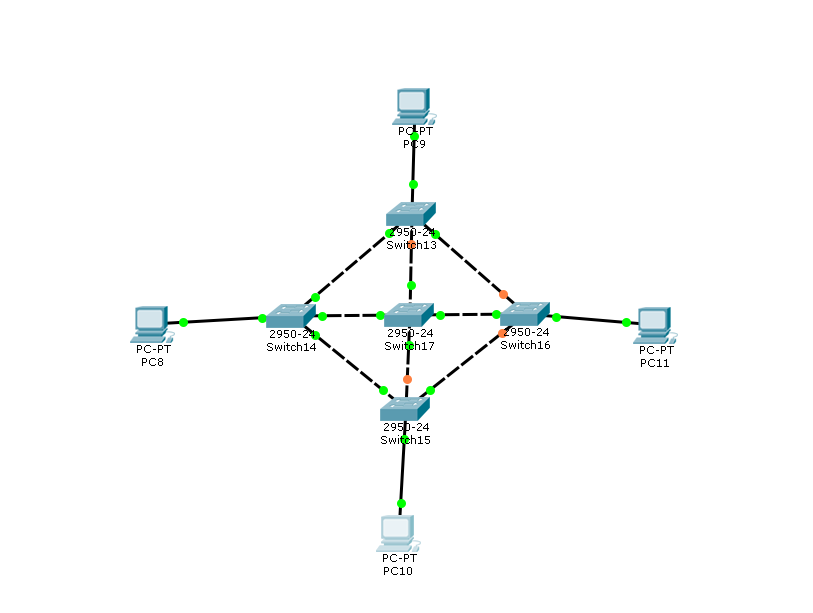
\includegraphics[scale=0.4]{images/ini.png}
    \caption{Red implementada inicialmente}
    \label{fig:my_label}
\end{figure}
\newpage
Luego, a los Switches que están marcados con naranjos se les aplica el protocolo STP, esto es netamente para ver que es lo que sucede con la red, para ello se implementa lo siguiente
\begin{figure}[h]
    \centering
    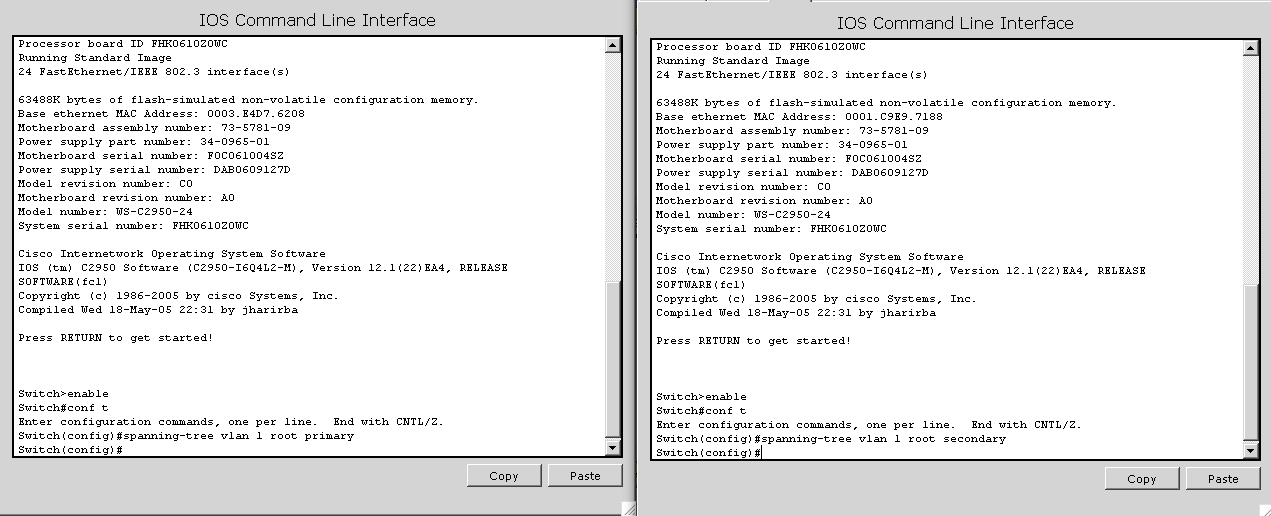
\includegraphics[scale=0.3]{images/cod.png}
    \caption{Códigos}
    \label{fig:my_label}
\end{figure}
\\Dando como resultado lo siguiente...
\begin{figure}[h]
    \centering
    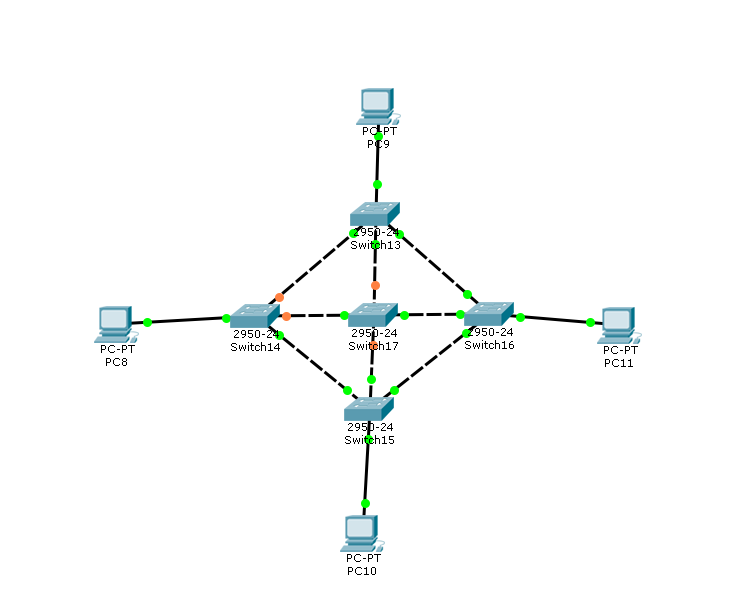
\includegraphics[scale=0.4]{images/modificado.png}
    \caption{Red implementada luego de modificarla}
    \label{fig:my_label}
\end{figure}
\newpage
Se puede observar que al dejar los Switches anteriormente marcados en naranjo como primarios y secundarios, a los cuales también se les asigna una prioridad, estos quedan marcados como verde, es decir se provoco una configuración en la red.
\\Posteriormente se realiza un Ping cuando se desactiva el protocolo de los switches para ver que es lo que sucede, arrojando como resultado:
\begin{figure}[h]
    \centering
    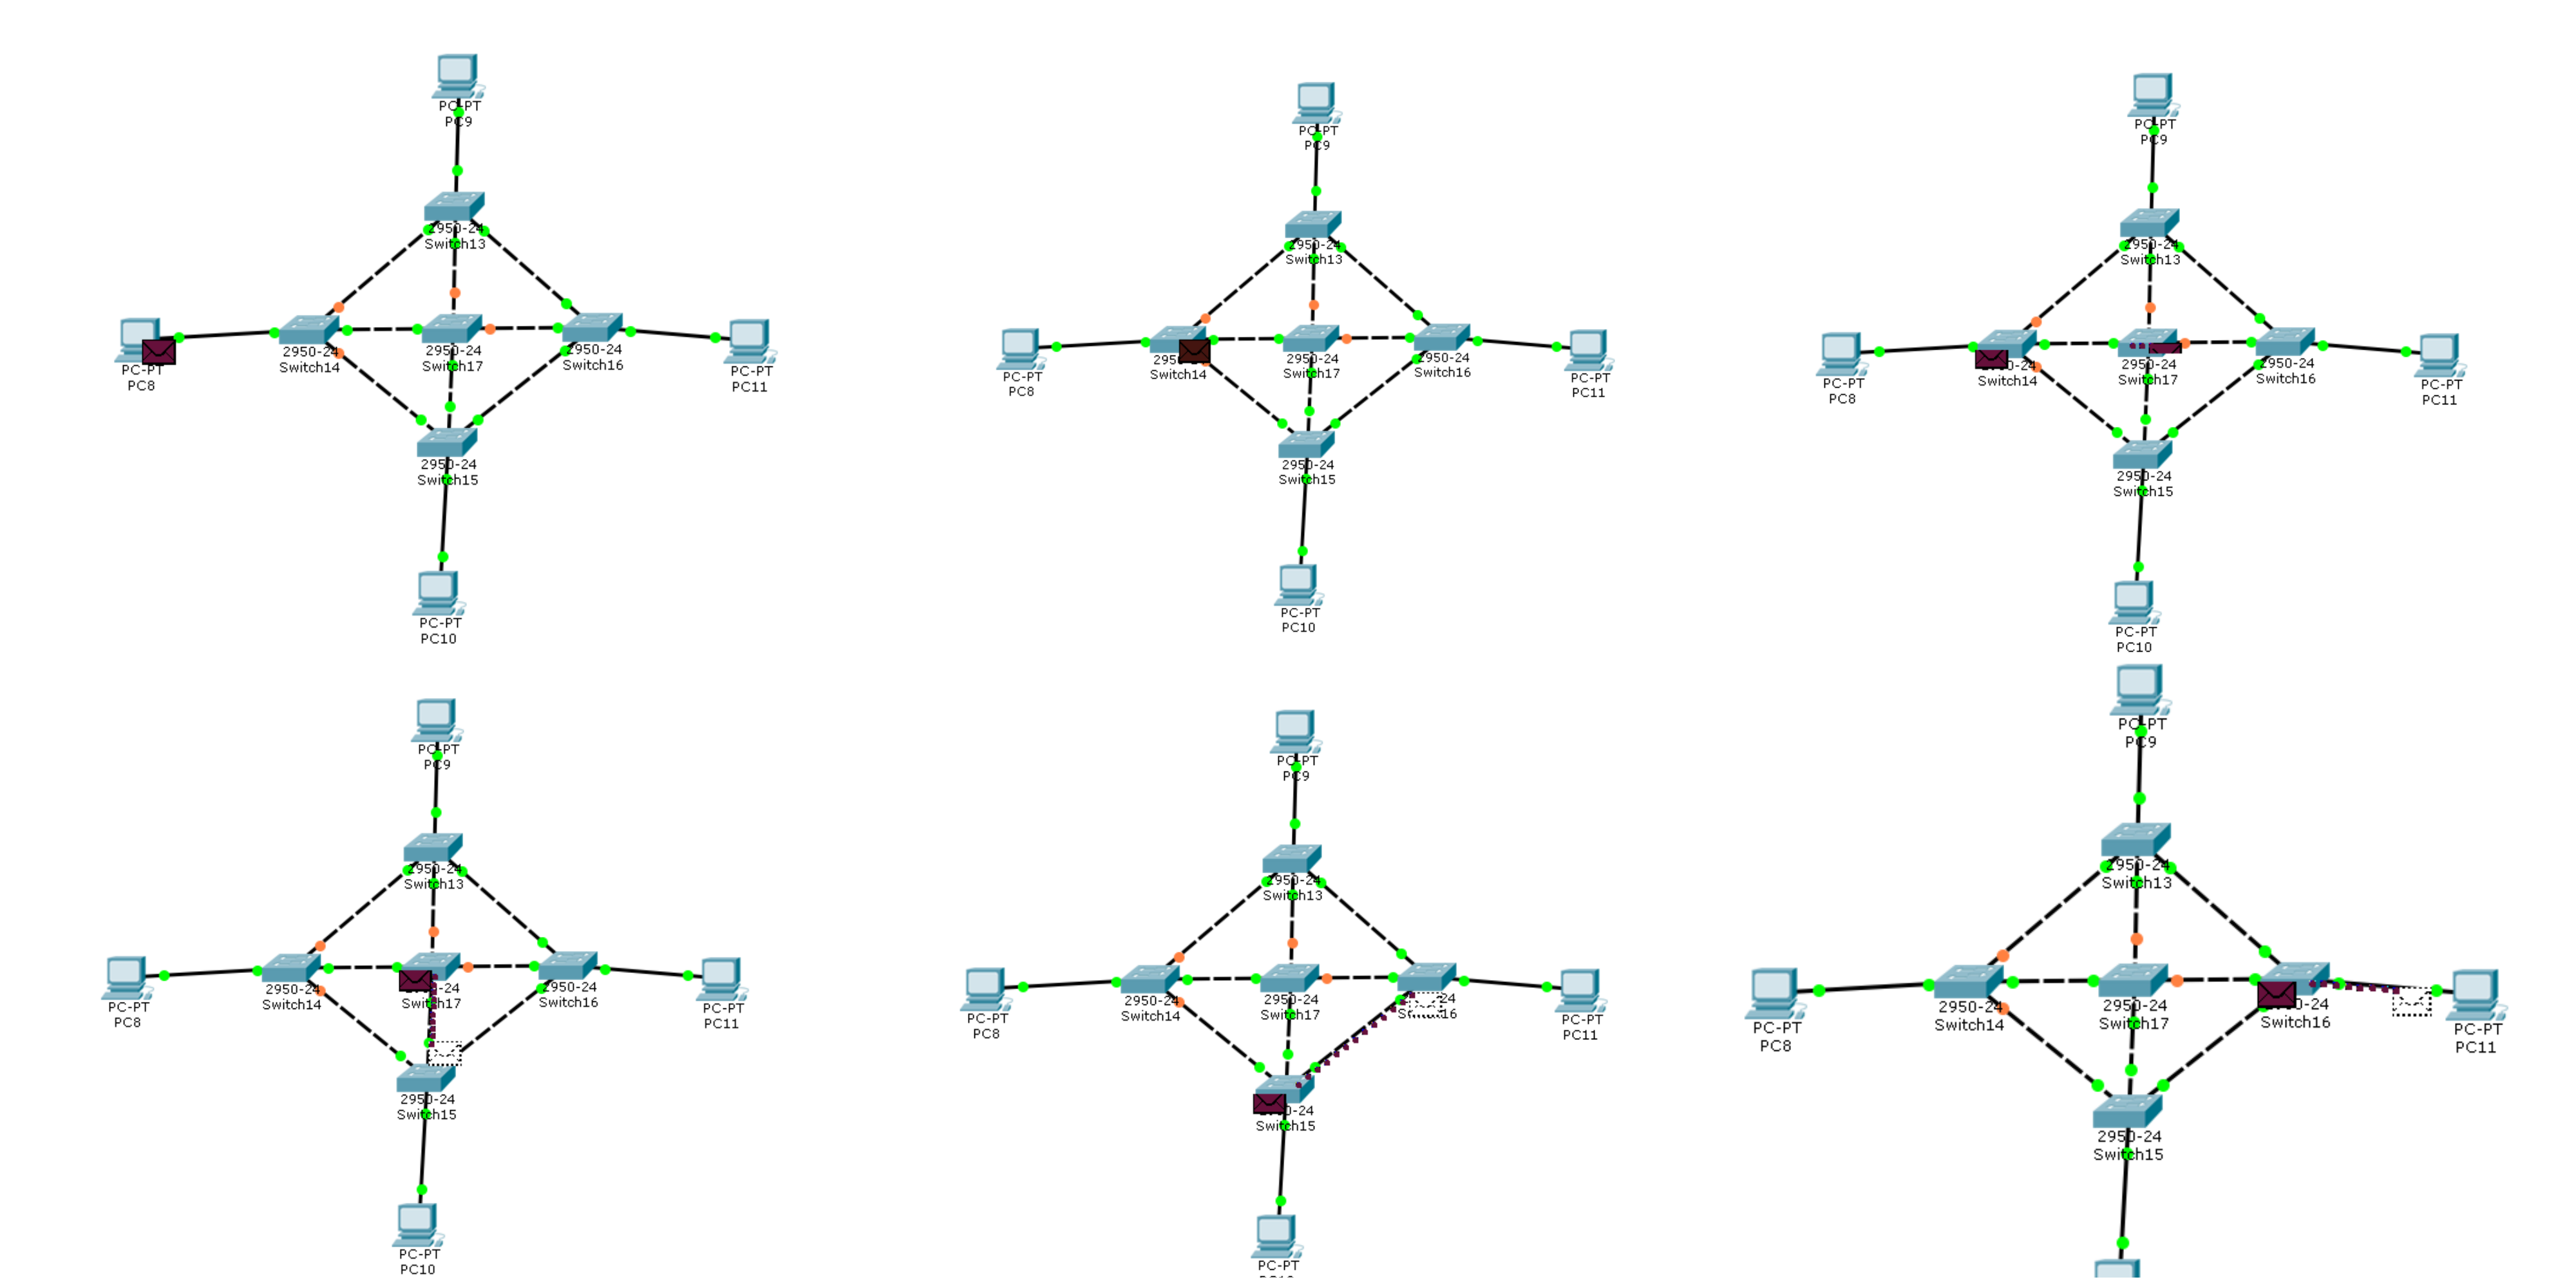
\includegraphics[scale=0.1]{images/1.png}
    \caption{Red implementada STP y envio de paquete}
    \label{fig:my_label}
\end{figure}
\section{Actividad 2}
Esta parte tiene como objetivo la creación de 4 VLANs, antes de empezar a implementar, se detallara a continuación el modelo de red a trabajar.
\begin{figure}[h]
    \centering
    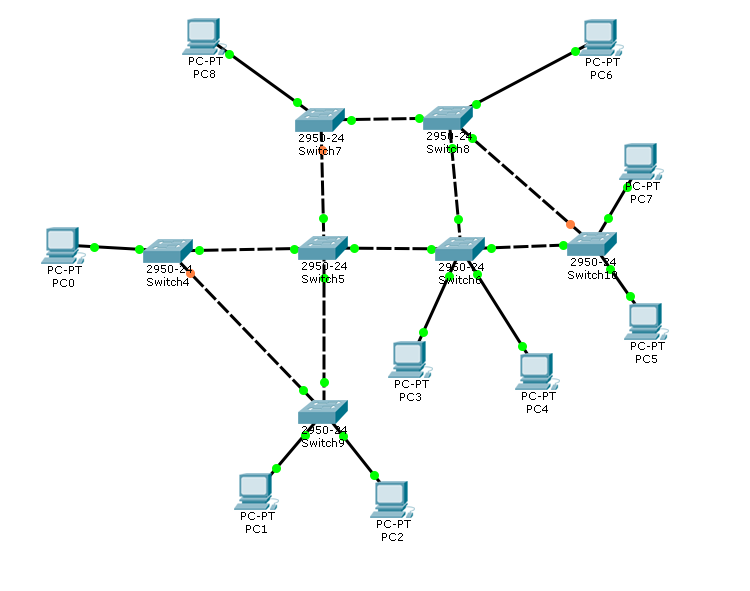
\includegraphics[scale=0.4]{images/inib.png}
    \caption{Red implementada inicialmente}
    \label{fig:my_label}
\end{figure}
\newpage
Lo central de esta actividad fue configurar todos los equipos con la finalidad de asignar las VLANs especificadas por el ayudante, para ello se utilizan los comandos proporcionados por el mismo para ir configurando cada Switch, junto con esto, tambien se habilitan los puertos como modo Trunk (switch-switch) o Access(pc-switch).
\begin{figure}[h]
    \centering
    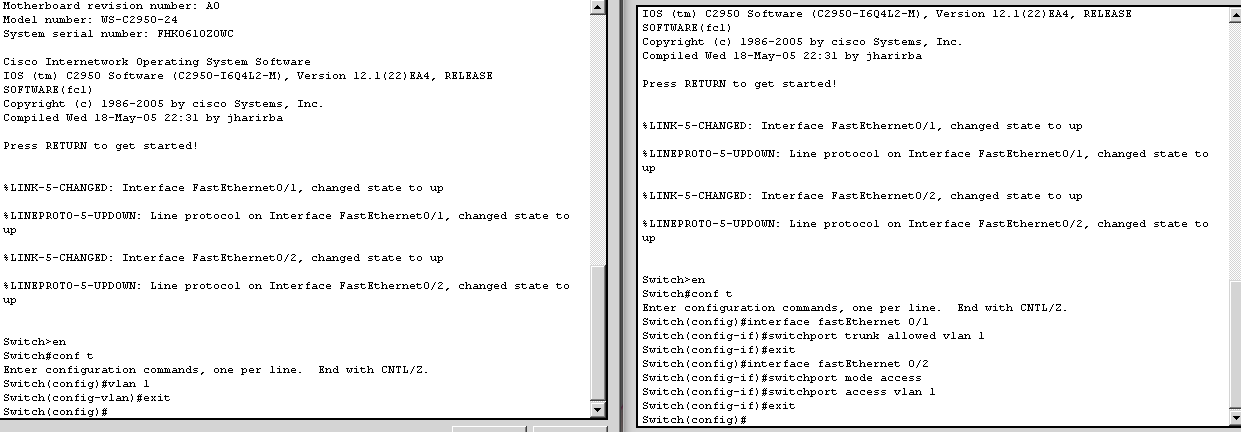
\includegraphics[scale=0.2]{images/3.png}
    \caption{Códigos}
    \label{fig:my_label}
\end{figure}
\\Finalmente, con todos los Switches conectados, se obtiene el siguiente resultado...
\begin{figure}[h]
    \centering
    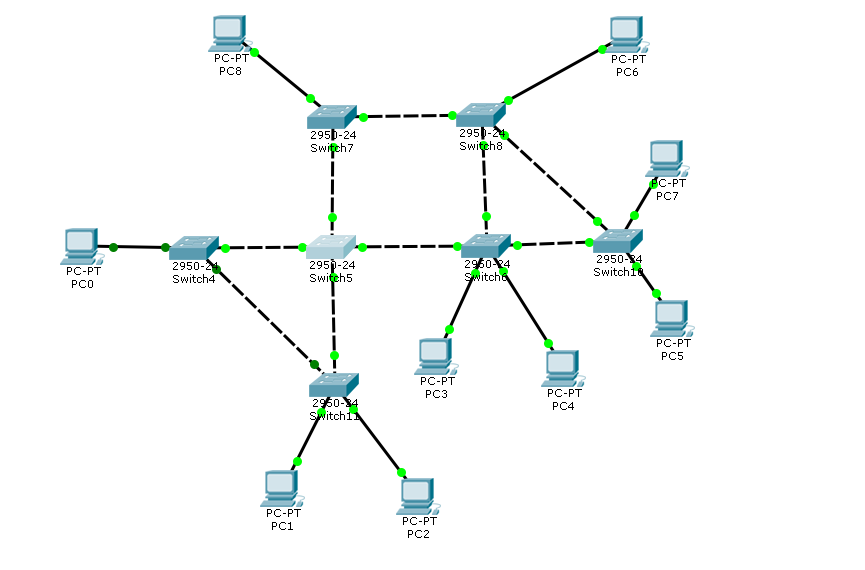
\includegraphics[scale=0.4]{images/4.png}
    \caption{Red implementada VLAN}
    \label{fig:my_label}
\end{figure}
 \\ Lo que evidencia la imagen al final, es que la red queda sin colisiones ya que todos los puntos de los puertos están de color verde.
\chapter{Cuestionario}
\begin{enumerate}
    \item ¿Cual es la diferencia entre modo Trunk y modo Access?
    La diferencia entre estos modos radica principalmente en la cantidad de VLANs que están conectadas, vale decir, modo Access pertenece a una única VLAN, en cambio, modo Trunk puede ser parte de muchas VLANs\\Otra diferencia es que en modo Access se usa para conectar a equipos finales, mientras que en modo Trunk se usa para conexiones entre switch
    \item ¿Que ocurre si conecto una puerta en modo Trunk a un PC?
    Por lo que se observa al realizar el cambio, el puerto de entrada conectado con el pc marca verde, lo que podría interpretarse como que el switch para ese puerto quedo como una única VLAN .
    \item ¿Que ruta sigue un ping del PC 3 al PC 8? ¿Es una ruta eficiente en
     cuanto a tiempo? ¿Que opción daría usted para poder llegar a los tres PC
     con VLAN 3 sin generar bucles y ser óptimo en tiempo?
     El PC3 esta en VLAN1, por lo que no llega el mensaje, ahora si conectamos el PC4 que es de la misma VLAN 3 que el PC8, el mensaje llegara por una ruta optima ya que va del switch 6->7->8 hasta llegar a su destino.
    \item ¿Que pasa si conecto dos switchs uno con la puerta Trunk y la otra con
     puerta Access?
     El puesto de switch marcara naranjo, esto se debe a que ese switch tomara una única vlan conectándose a como lo hace un computador.
    \item ¿Cuales son las ventajas de este sistema llamado VLAN? Mencione al
     menos 3.
     \begin{itemize}
         \item Mejora el rendimiento de la red
         \item Menos costo ya que no requiere actualizar a una red nueva
         \item Mitiga tormenta Broadcast
     \end{itemize}


\end{enumerate}

\chapter{Conclusión}
Del presente informe se concluye que el trabajo con los protocolos de Switch STP y VLAN en una red con redundancias fue efectivo para los modelos que propusieron, viéndose de manera practica los resultados y diferencias que implicaba o no tener estos protocolos, como se muestra en la actividad practica, los objetivos se cumplieron ya que como se ilustran en las imágenes se nota una gran diferencia de antes y después de haber configurado los switches con STP o bien VLAN asignados para la red implementada.
\\ Finalmente, se tiene que el conocimiento practico del funcionamiento de estas redes es fundamental para comprender la teoría vista en cátedra sobre STP y VLAN.
\begin{thebibliography}{0}
\bibitem{1}Introducción y configuración de STP. Recuperado de: \\ \url{https://www.cisco.com/c/es_mx/support/docs/lan-switching/spanning-tree-protocol/5234-5.html}
\bibitem{2}que es una VLAN y su funcionamiento. Recuperado de: \\
\url{http://redesconfiguracion.blogspot.cl/2015/07/que-es-una-vlan-y-su-funcion.html}
\end{thebibliography}
\listoffigures
\end{document}

